\documentclass[11pt]{article}
\usepackage{amsmath,amsbsy,amssymb,verbatim,fullpage,ifthen,graphicx,bm,amsfonts,amsthm,url}
\usepackage{graphicx}
\usepackage{xcolor}
\usepackage{caption}
\usepackage{subcaption}
\usepackage{listings}

\newcommand{\mfile}[1]  {{\small \verbatiminput{./#1}}} % Jeff Fessler, input matlab file
\newcommand{\tmop}[1]{\ensuremath{\operatorname{#1}}}
%\newcommand*{\qed}{\hfill\ensuremath{\blacksquare}}%
\newcommand{\R}{\mathbb{R}}
\newcommand{\C}{\mathbb{C}}
\newcommand{\Z}{\mathbb{Z}}
\newcommand{\A}{\mathcal{A}}
\newcommand{\minimize}{\operatorname*{minimize\ }}
\newcommand{\maximize}{\operatorname*{maximize}}
\newcommand{\opdet}[1]{\operatorname{\textbf{det}}\left(#1\right)}
\newcommand{\optr}[1]{\operatorname{\textbf{tr}}\left(#1\right)}
%\newcommand{\AnswerDefine}{}
\newcommand{\answer}[2][blue]{\ifdefined\AnswerDefine{\color{#1}\it#2}\fi}
\newcommand{\mtx}[1]{\mathbf{#1}}
\newcommand{\vct}[1]{\mathbf{#1}}
\def \lg       {\langle}
\def \rg       {\rangle}
\def \mA {\mtx{A}}
\def \mF {\mtx{F}}
\def \mG {\mtx{G}}
\def \mI {\mtx{I}}
\def \mJ {\mtx{J}}
\def \mU {\mtx{U}}
\def \mS {\mtx{S}}
\def \mV {\mtx{V}}
\def \mW {\mtx{W}}
\def \mLambda {\mtx{\Lambda}}
\def \mSigma {\mtx{\Sigma}}
\def \mX {\mtx{X}}
\def \mY {\mtx{Y}}
\def \mZ {\mtx{Z}}
\def \zero     {\mathbf{0}}
\def \vzero    {\vct{0}}
\def \vone    {\vct{1}}
\def \va {\vct{a}}
\def \vg {\vct{g}}
\def \vu {\vct{u}}
\def \vv {\vct{v}}
\def \vx {\vct{x}}
\def \vy {\vct{y}}
\def \vz {\vct{z}}
\def \vphi {\vct{\phi}}
\def \vmu {\vct{\mu}}
\def \R {\mathbb{R}}

%\newcommand{\st}{\operatorname*{\ subject\ to\ }}
\usepackage{algorithm,algpseudocode}
\usepackage{xspace}
% Add a period to the end of an abbreviation unless there's one
% already, then \xspace.
\makeatletter
\DeclareRobustCommand\onedot{\futurelet\@let@token\@onedot}
\def\@onedot{\ifx\@let@token.\else.\null\fi\xspace}

\def\eg{\emph{e.g}\onedot} \def\Eg{\emph{E.g}\onedot}
\def\ie{\emph{i.e}\onedot} \def\Ie{\emph{I.e}\onedot}
\def\cf{\emph{c.f}\onedot} \def\Cf{\emph{C.f}\onedot}
\def\etc{\emph{etc}\onedot} \def\vs{\emph{vs}\onedot}
\def\wrt{w.r.t\onedot} \def\dof{d.o.f\onedot}
\def\etal{\emph{et al}\onedot} \def\st{\emph{s.t}\onedot}
\pagestyle{plain}

\title{{\bf Homework Set 6, CPSC 8420, Fall 2024}} % Change to the appropriate homework number
\author{\Large\underline{Collins, Matthew}}
\date{\textbf{\Large\textcolor{red}{Due 12/05/2024, 11:59PM EST}}} % put your name in the LastName, FirstName format
%\date{\today}

\begin{document}
\maketitle


\section*{Problem 1}
Frequently, the affinity matrix is constructed as:
\begin{equation}
	A_{ij}=e^{-d(x_i,x_j)^2/\sigma}
\end{equation}
where $\sigma$  is some user-specified parameter. The best that we can hope for in practice is a near block-diagonal
affinity matrix. It can be shown in this case, that after projecting to the space spanned by the top $k$
eigenvectors, points which belong to the same block are close to each other in a euclidean sense. The steps are as follows:
\begin{itemize}
	\item Construct an affinity matrix $A$ using the above equation.
	\item Symmetrically `normalize’ the rows and columns of $A$ to get a matrix $N$ such that $N(i,j)=\frac{A(i,j)}{\sqrt{d(i)d(j)}}$, where $d(i)=\sum_k A(i,k)$.
	\item Construct a matrix $Y$ whose columns are the first $k$ eigenvectors of $N$.
	\item Normalize each row of $Y$ such that it is of unit length.
	\item Cluster the dataset by running $k$-means on the set of  embedded points, where each row of $Y$ is a data-point.
\end{itemize}

\begin{enumerate}
	\item Run $k$-means on the datasets provided in the .zip file. For text.mat, take $k = 6$. For all others use $k = 2$.
	\item  Implement the above spectral clustering algorithm and run it on the four provided datasets using the same $k$. Plot your clustering results using $\sigma = .025, .05, .2, .5$. Hints: You may find the MATLAB functions pdist and eig to be helpful. A function plotClusters.m has been provided to help visualize clustering results.
	\item Plot the first 10 eigenvalues for the rectangles.mat and text.mat datasets when $\sigma = .05$. What do you notice?
	\item How do $k$-means and spectral clustering compare?
\end{enumerate}
\begin{figure}[h!]
	\centering
	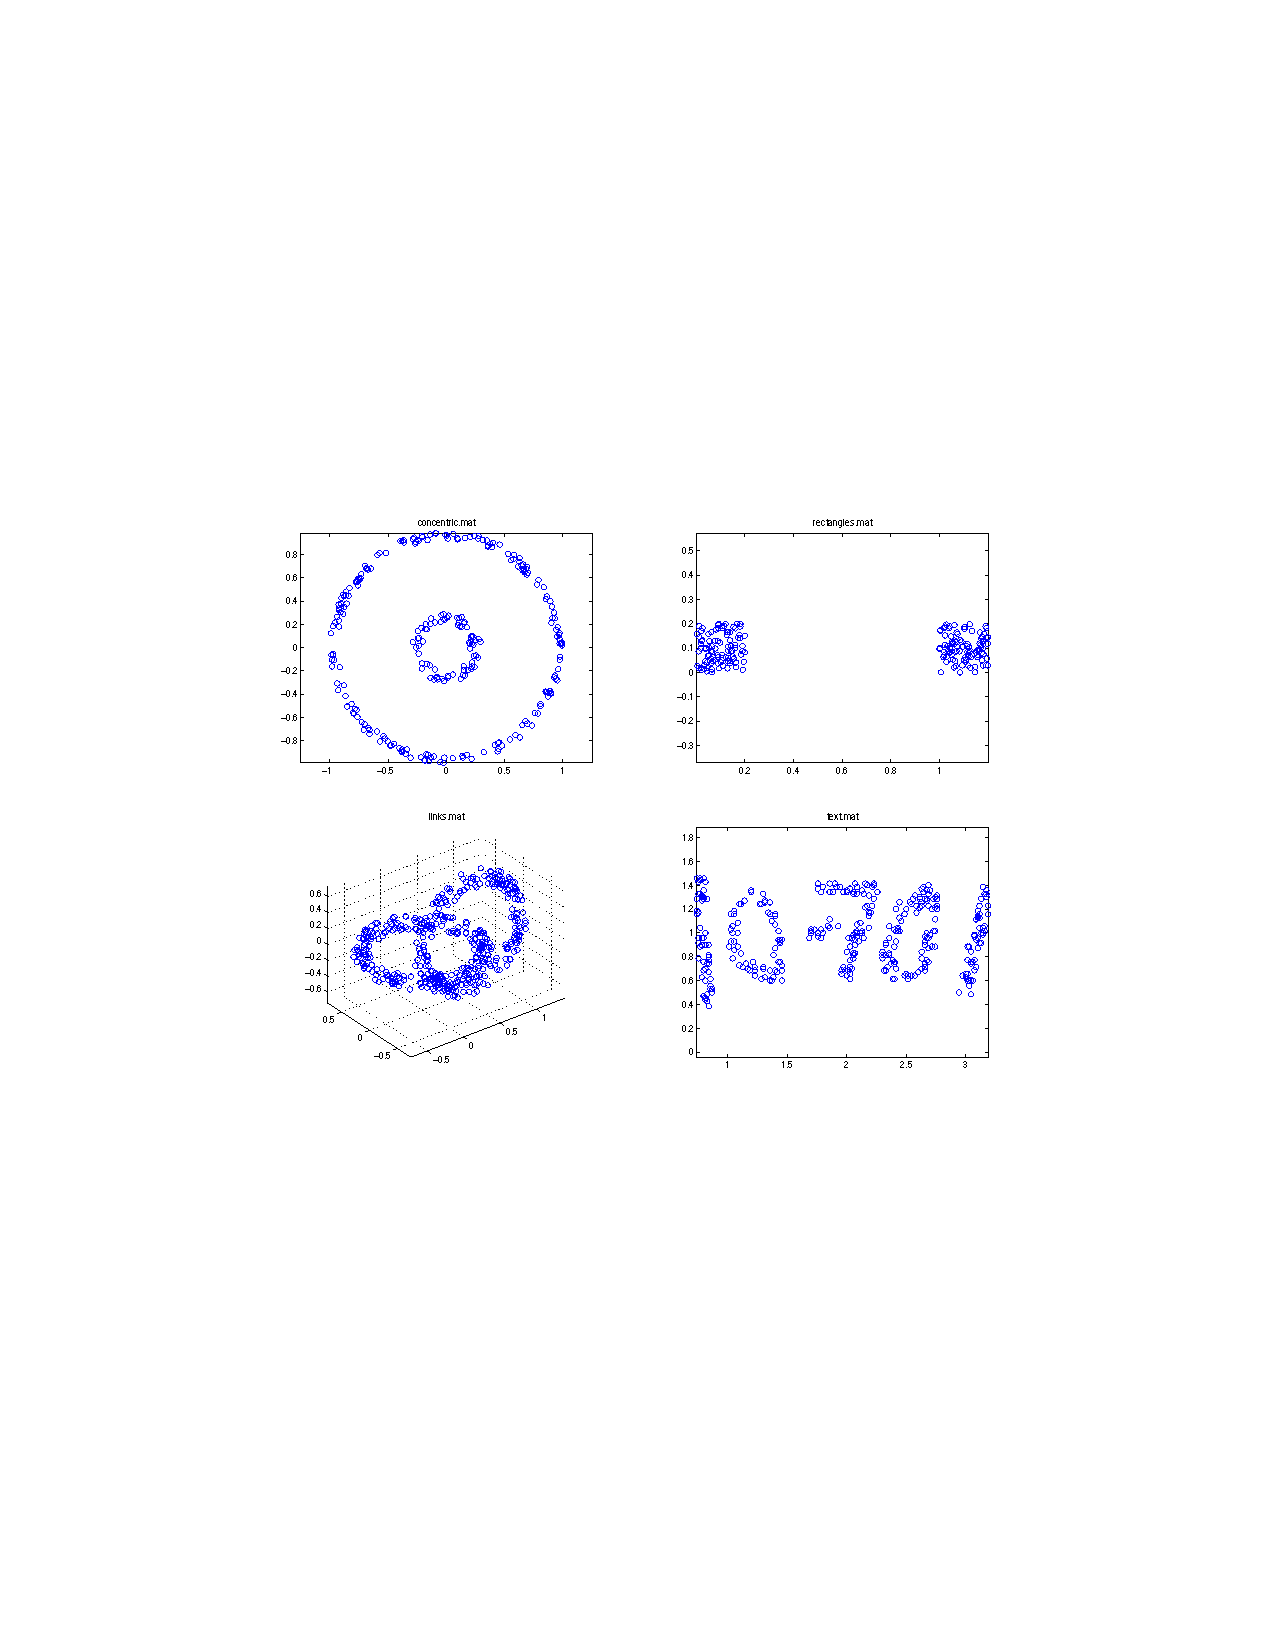
\includegraphics[width=\linewidth]{syn}
\end{figure}

\clearpage
\textcolor{red}{P1.1, Answer:}\\

The clustering algorithm groups the data into k clusters, where k=6 for text.mat and k=2 for the other datasets.
\begin{figure}[!ht]
    \centering
    \begin{subfigure}{0.45\textwidth}
        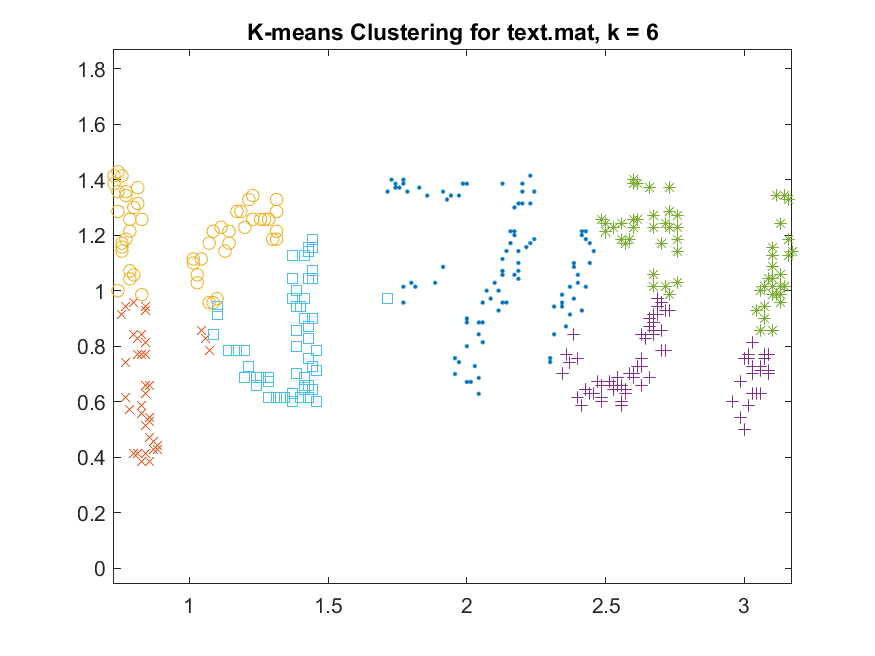
\includegraphics[width=\linewidth]{k_means_clustering_text.mat.png}
        \caption{K-means clustering for \texttt{text.mat}}
    \end{subfigure}
    \begin{subfigure}{0.45\textwidth}
        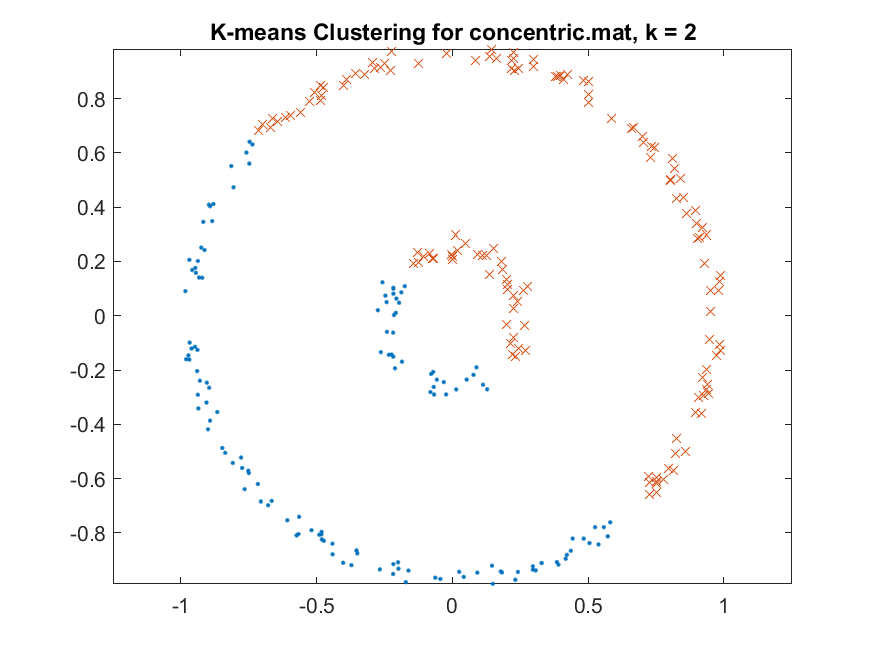
\includegraphics[width=\linewidth]{k_means_clustering_concentric.mat.png}
        \caption{K-means clustering for \texttt{concentric.mat}}
    \end{subfigure}
    \begin{subfigure}{0.45\textwidth}
        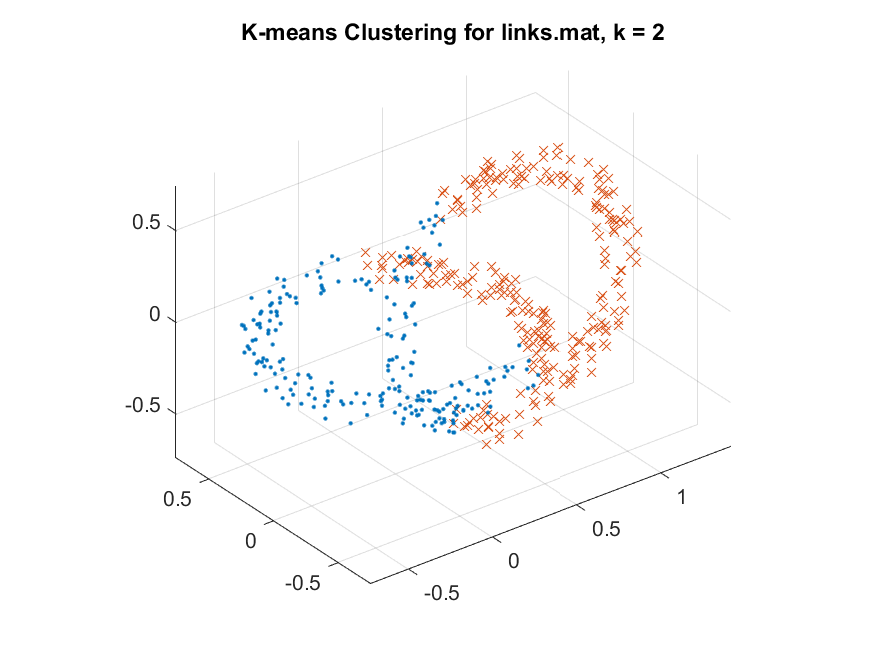
\includegraphics[width=\linewidth]{k_means_clustering_links.mat.png}
        \caption{K-means clustering for \texttt{links.mat}}
    \end{subfigure}
    \begin{subfigure}{0.45\textwidth}
        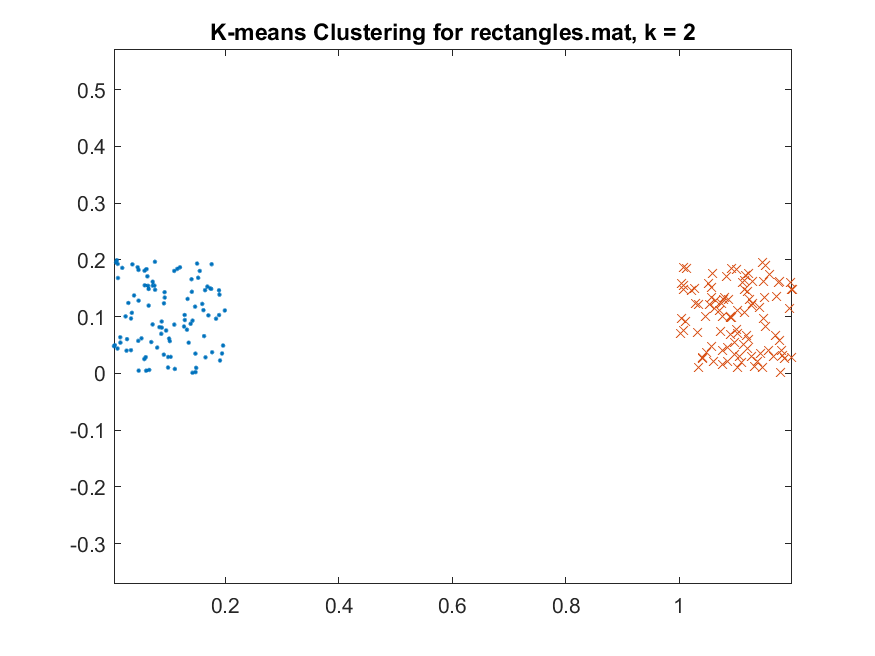
\includegraphics[width=\linewidth]{k_means_clustering_rectangles.mat.png}
        \caption{K-means clustering for \texttt{rectangles.mat}}
    \end{subfigure}
    \caption{K-means clustering results for the provided datasets.}
    \label{fig:kmeans}
\end{figure}





\textcolor{red}{P1.2, Answer:}\\

The \texttt{rectangles.mat} dataset exhibits two clearly separated clusters, and spectral clustering is largely insensitive to the value of \(\sigma\). Across all tested \(\sigma\) values, the clusters are correctly identified, reflecting the dataset's inherent simplicity and large separation between clusters. Even with a large \(\sigma\), where global similarities dominate, the clustering remains accurate due to the strong geometric distinction between the rectangles.

\begin{figure}[!ht]
    \centering
    \begin{subfigure}{0.45\textwidth}
        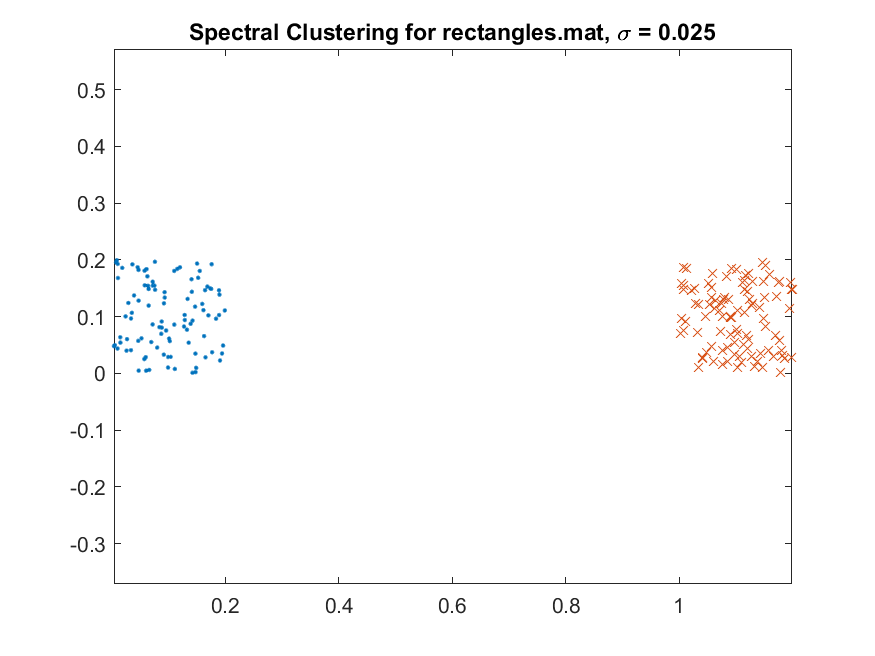
\includegraphics[width=\linewidth]{rectangles_sigma_0.025.png}
        \caption{\(\sigma = 0.025\)}
    \end{subfigure}
    \begin{subfigure}{0.45\textwidth}
        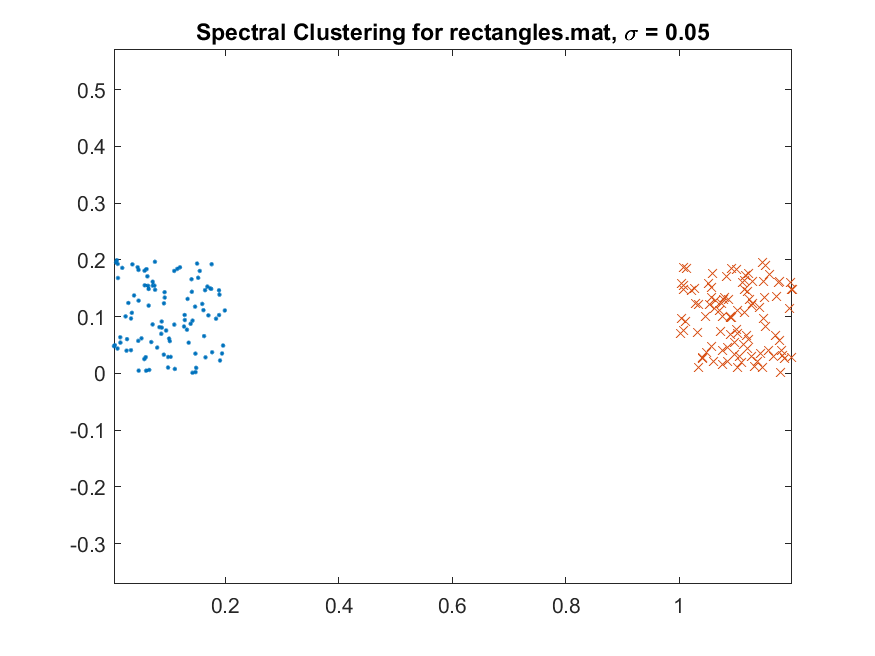
\includegraphics[width=\linewidth]{rectangles_sigma_0.050.png}
        \caption{\(\sigma = 0.05\)}
    \end{subfigure}
    \begin{subfigure}{0.45\textwidth}
        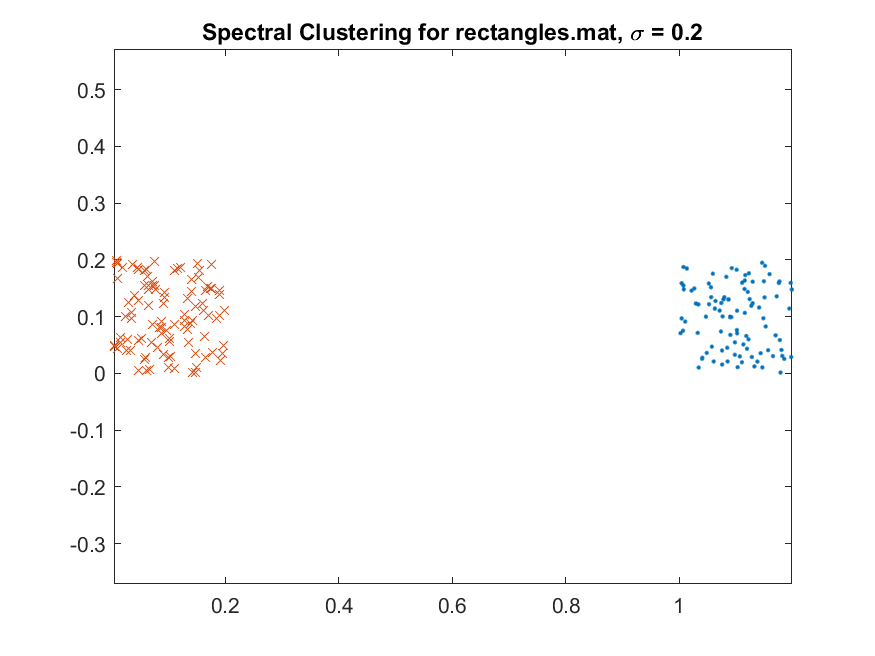
\includegraphics[width=\linewidth]{rectangles_sigma_0.200.png}
        \caption{\(\sigma = 0.2\)}
    \end{subfigure}
    \begin{subfigure}{0.45\textwidth}
        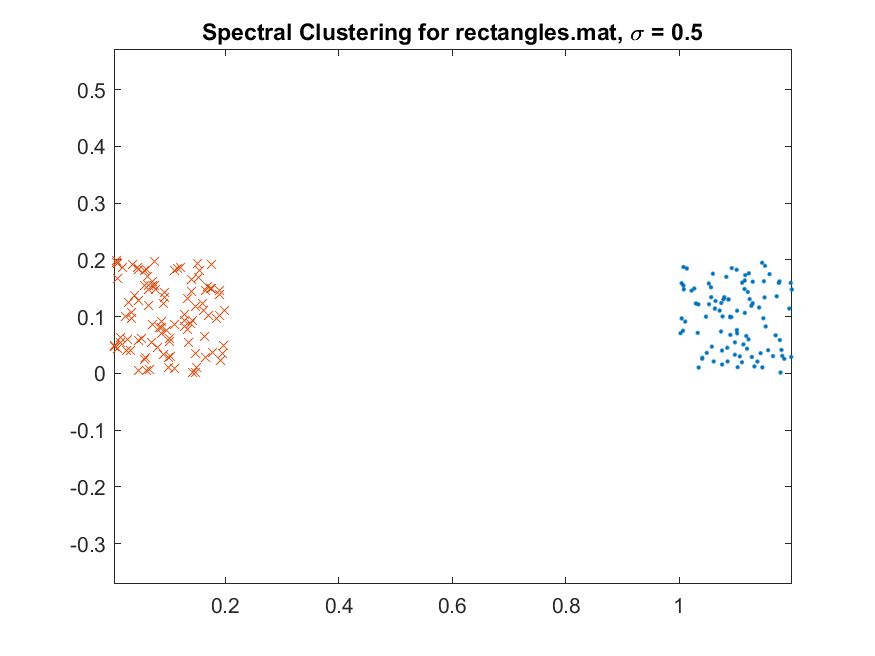
\includegraphics[width=\linewidth]{rectangles_sigma_0.500.png}
        \caption{\(\sigma = 0.5\)}
    \end{subfigure}
    \caption{Spectral clustering results for \texttt{rectangles.mat} with varying \(\sigma\).}
    \label{fig:rectangles}
\end{figure}

The \texttt{links.mat} dataset has two intertwined clusters, making it more sensitive to changes in \(\sigma\). For smaller \(\sigma\) values (\(0.025\) and \(0.05\)), the clustering is highly accurate, as the algorithm emphasizes local neighborhood relationships. As \(\sigma\) increases (\(0.2\) and \(0.5\)), global similarities blur the cluster boundaries, resulting in some misclassification near the overlap of the "links."

\begin{figure}[!ht]
    \centering
    \begin{subfigure}{0.45\textwidth}
        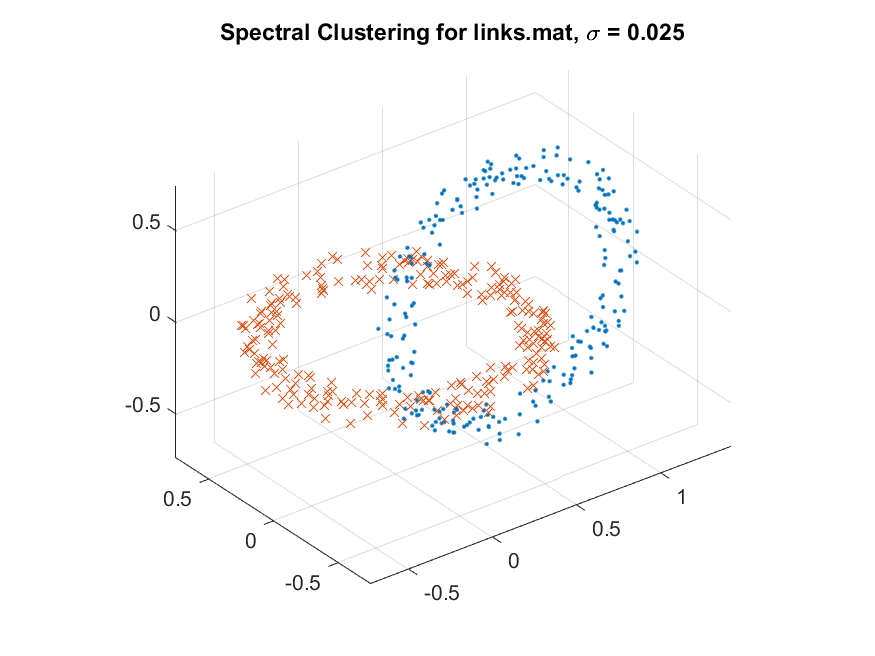
\includegraphics[width=\linewidth]{links_sigma_0.025.png}
        \caption{\(\sigma = 0.025\)}
    \end{subfigure}
    \begin{subfigure}{0.45\textwidth}
        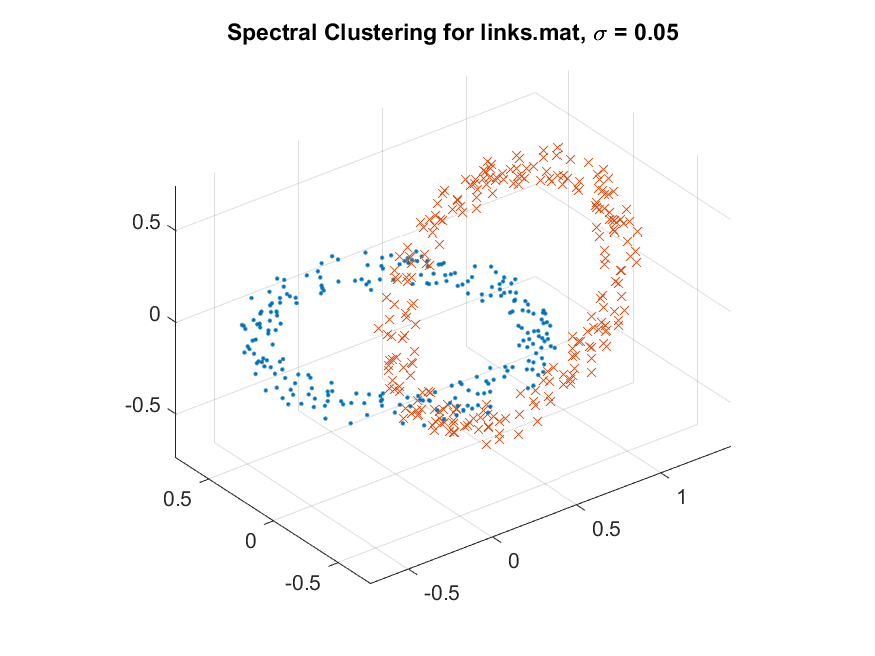
\includegraphics[width=\linewidth]{links_sigma_0.050.png}
        \caption{\(\sigma = 0.05\)}
    \end{subfigure}
    \begin{subfigure}{0.45\textwidth}
        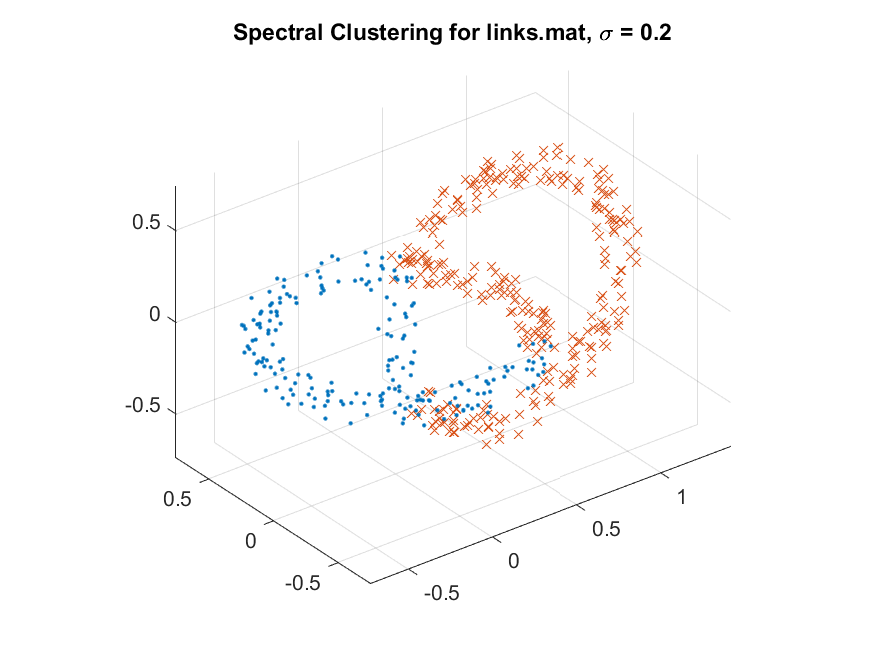
\includegraphics[width=\linewidth]{links_sigma_0.200.png}
        \caption{\(\sigma = 0.2\)}
    \end{subfigure}
    \begin{subfigure}{0.45\textwidth}
        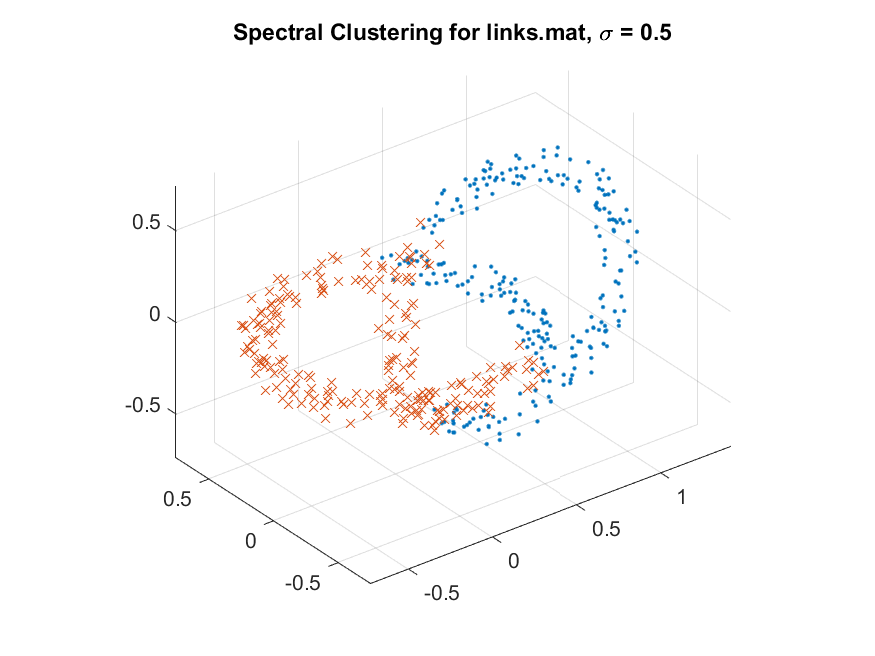
\includegraphics[width=\linewidth]{links_sigma_0.500.png}
        \caption{\(\sigma = 0.5\)}
    \end{subfigure}
    \caption{Spectral clustering results for \texttt{links.mat} with varying \(\sigma\).}
    \label{fig:links}
\end{figure}

The \texttt{concentric.mat} dataset shows the importance of \(\sigma\) in clustering performance. For smaller \(\sigma\) values (\(0.025\) and \(0.05\)), the clustering is highly accurate, as local similarities dominate, allowing the algorithm to distinguish between the two concentric rings. As \(\sigma\) increases (\(0.2\) and \(0.5\)), the clusters become less distinct, and points from different rings begin to influence each other, leading to errors.

\begin{figure}[!ht]
    \centering
    \begin{subfigure}{0.45\textwidth}
        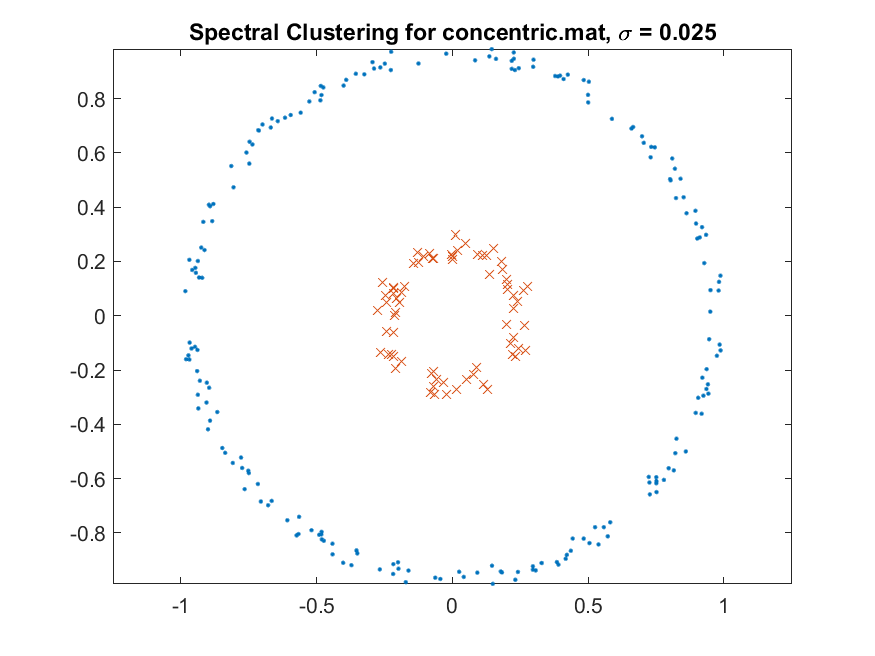
\includegraphics[width=\linewidth]{concentric_sigma_0.025.png}
        \caption{\(\sigma = 0.025\)}
    \end{subfigure}
    \begin{subfigure}{0.45\textwidth}
        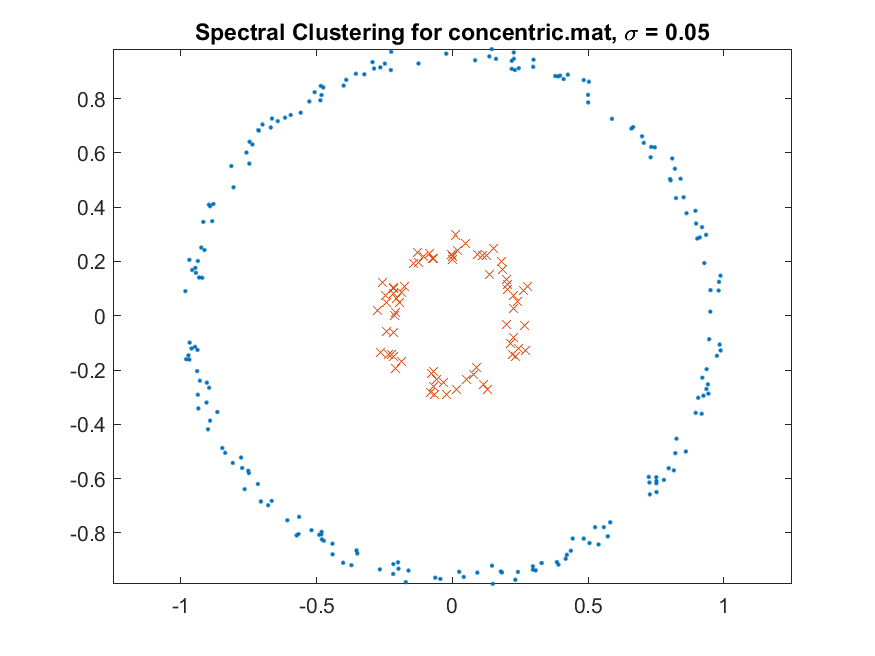
\includegraphics[width=\linewidth]{concentric_sigma_0.050.png}
        \caption{\(\sigma = 0.05\)}
    \end{subfigure}
    \begin{subfigure}{0.45\textwidth}
        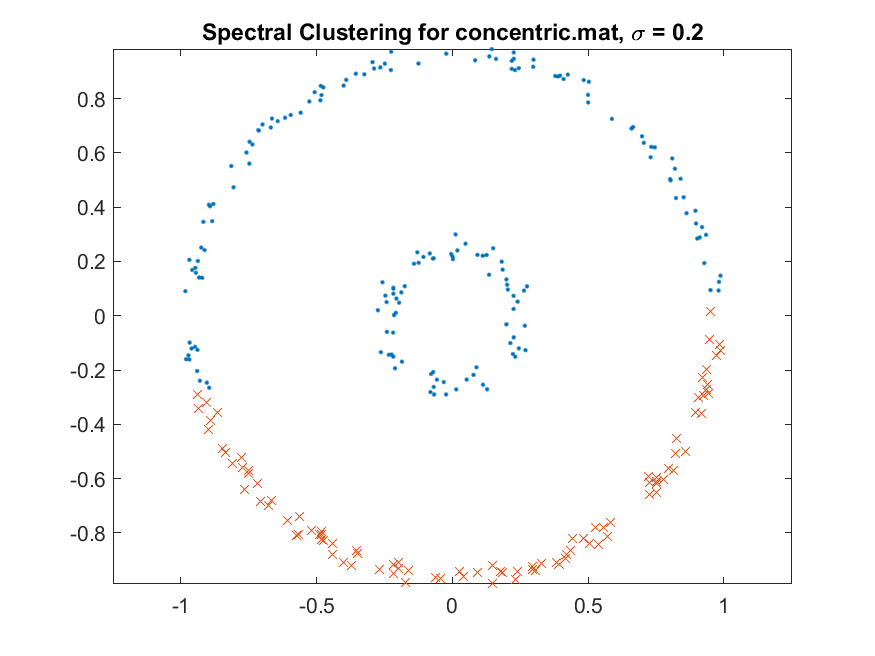
\includegraphics[width=\linewidth]{concentric_sigma_0.200.png}
        \caption{\(\sigma = 0.2\)}
    \end{subfigure}
    \begin{subfigure}{0.45\textwidth}
        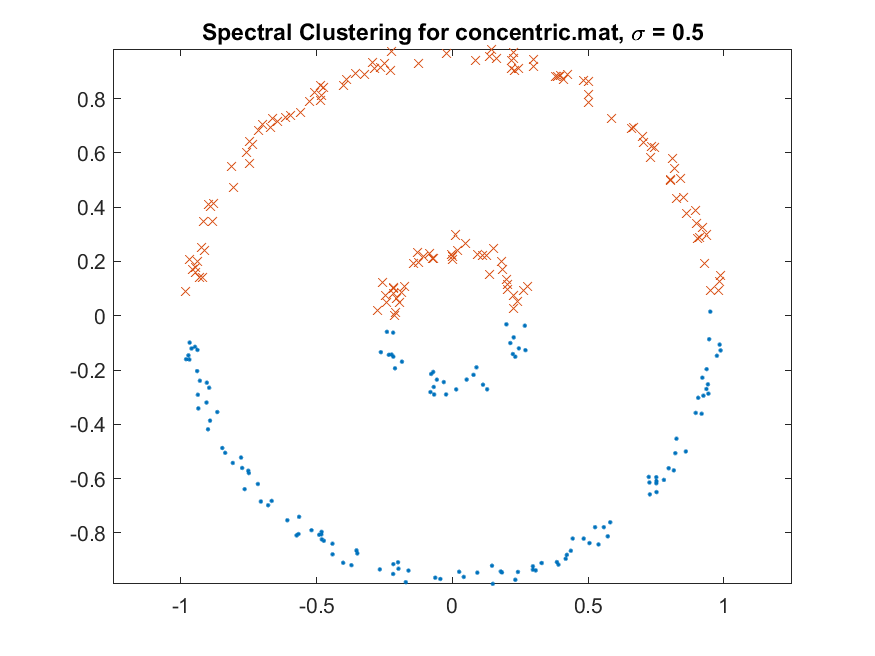
\includegraphics[width=\linewidth]{concentric_sigma_0.500.png}
        \caption{\(\sigma = 0.5\)}
    \end{subfigure}
    \caption{Spectral clustering results for \texttt{concentric.mat} with varying \(\sigma\).}
    \label{fig:concentric}
\end{figure}

The \texttt{text.mat} dataset demonstrates the importance of \(\sigma\) in separating six distinct clusters that correspond to different groups. 
At smaller \(\sigma\)\(=\)\(0.025\) the clustering is fairly well definied. Slight overlap is visible between cluster 1 and cluster 2, but the clusters are otherwise well separated. 
At \(\sigma\)\(=\)\(0.05\), the clustering is still pretty well-defined, but the algorithm begins to identify unintened clusters. Increasing the total number of 
cluster from the correct number of five to seven. As \(\sigma\) increases (\(0.2\) and \(0.5\)), the clustering becomes less accurate, with more clusters beginning to merge or become noisy. 
The sensitivity of this dataset highlights how spectral clustering relies on the proper choice of \(\sigma\) to emphasize local relationships while avoiding excessive smoothing.\\

\begin{figure}[!ht]
    \centering
    \begin{subfigure}{0.45\textwidth}
        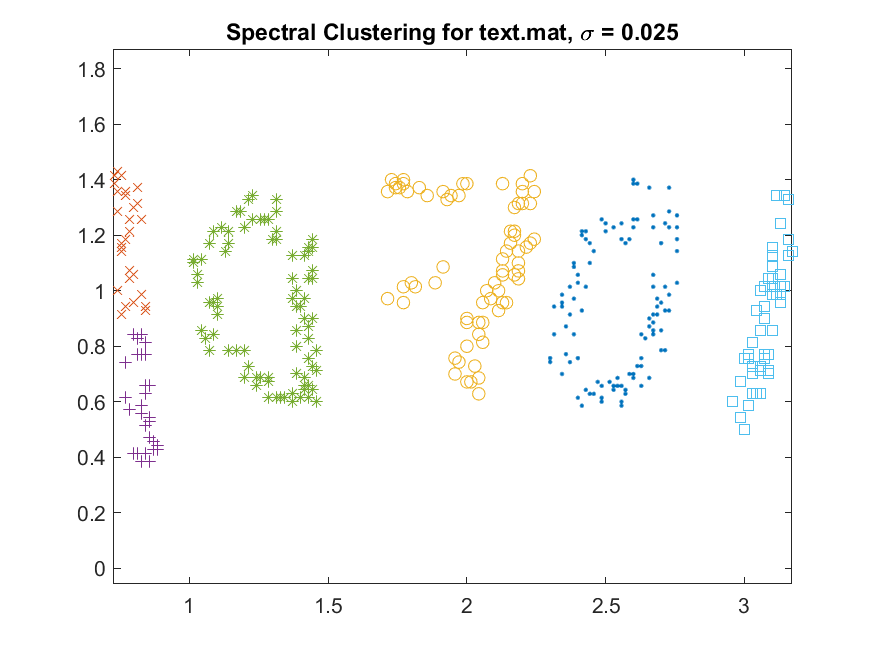
\includegraphics[width=\linewidth]{text_sigma_0.025.png}
        \caption{\(\sigma = 0.025\)}
    \end{subfigure}
    \begin{subfigure}{0.45\textwidth}
        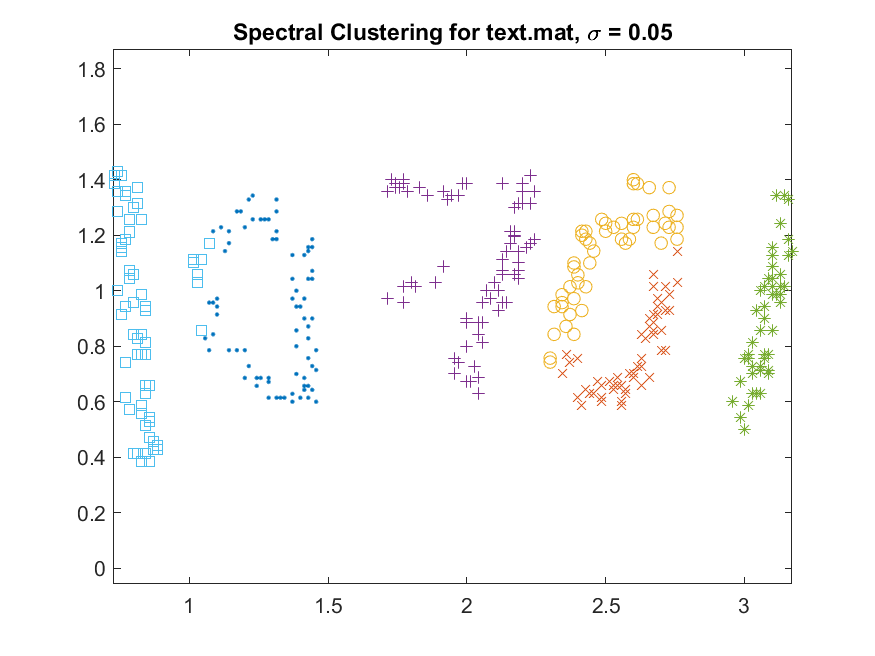
\includegraphics[width=\linewidth]{text_sigma_0.050.png}
        \caption{\(\sigma = 0.05\)}
    \end{subfigure}
    \begin{subfigure}{0.45\textwidth}
        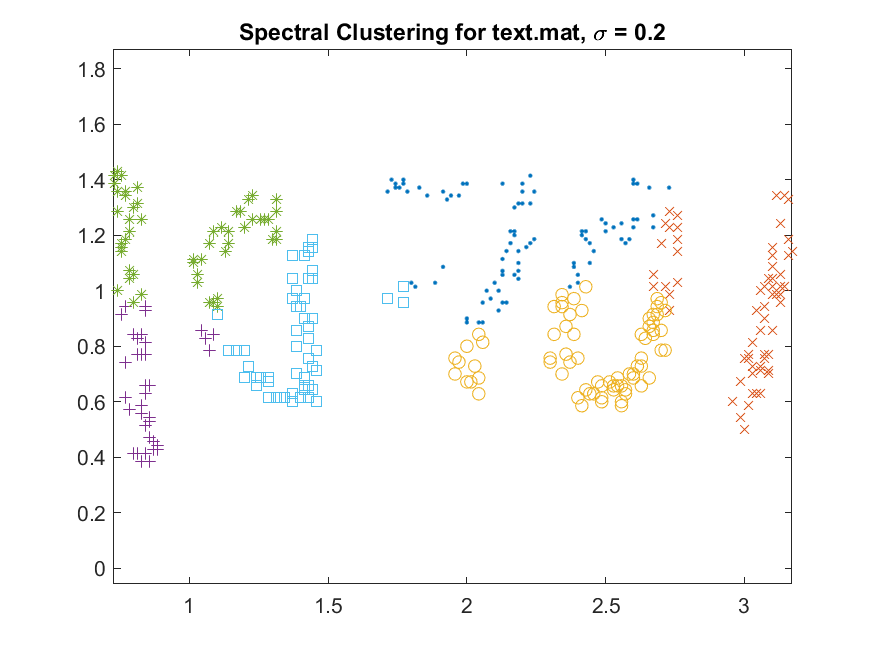
\includegraphics[width=\linewidth]{text_sigma_0.200.png}
        \caption{\(\sigma = 0.2\)}
    \end{subfigure}
    \begin{subfigure}{0.45\textwidth}
        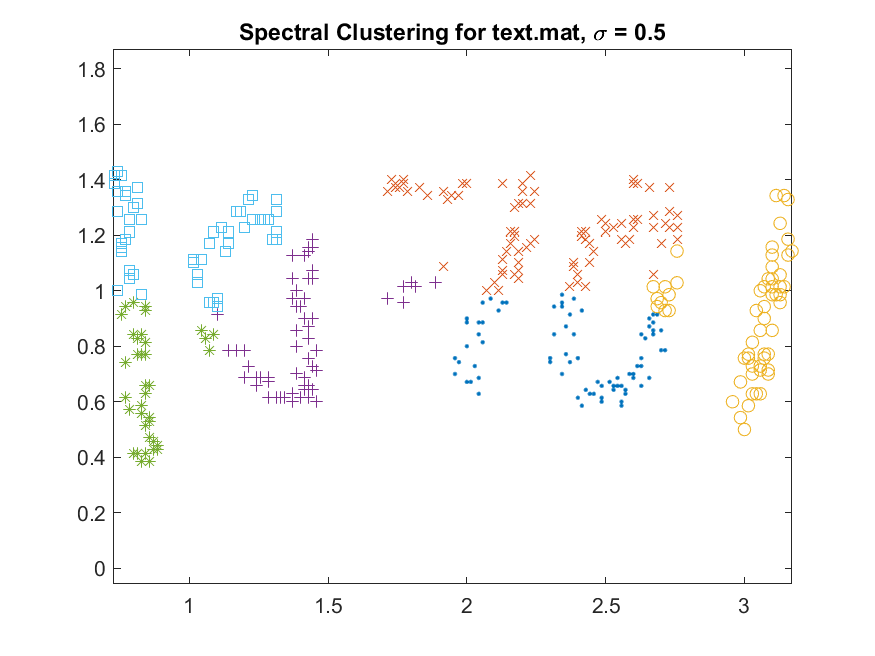
\includegraphics[width=\linewidth]{text_sigma_0.500.png}
        \caption{\(\sigma = 0.5\)}
    \end{subfigure}
    \caption{Spectral clustering results for \texttt{text.mat} with varying \(\sigma\).}
    \label{fig:text}
\end{figure}

\clearpage
\textcolor{red}{P1.3, Answer:}\\

The plots of the top 10 eigenvalues for \texttt{rectangles.mat} and \texttt{text.mat} in Figure \ref{fig:rectangles} reveal distinct differences in their clustering structure when \(\sigma = 0.05\).
For \texttt{rectangles.mat}, there is a sharp spectral gap between the second and third eigenvalues. The first two eigenvalues are significantly larger, 
indicating the presence of two dominant clusters in the dataset. This aligns with the expectation, as \texttt{rectangles.mat} contains two well-separated rectangular clusters. 
The remaining eigenvalues are close to zero, suggesting that most of the data's variance is captured by the first two eigenvectors, which correspond to the two clusters.
In contrast, the eigenvalues for \texttt{text.mat} show a gradual decrease, with no distinct spectral gap. This indicates that the dataset has a more complex structure and 
does not have well-separated clusters. Instead, the clusters may overlap, requiring more eigenvectors to adequately represent the data. The gradual decline in eigenvalues 
suggests that the clustering quality might depend heavily on the choice of parameters such as \(\sigma\) or \(k\).


\begin{figure}[!ht]
    \centering
    \begin{subfigure}{0.45\textwidth}
        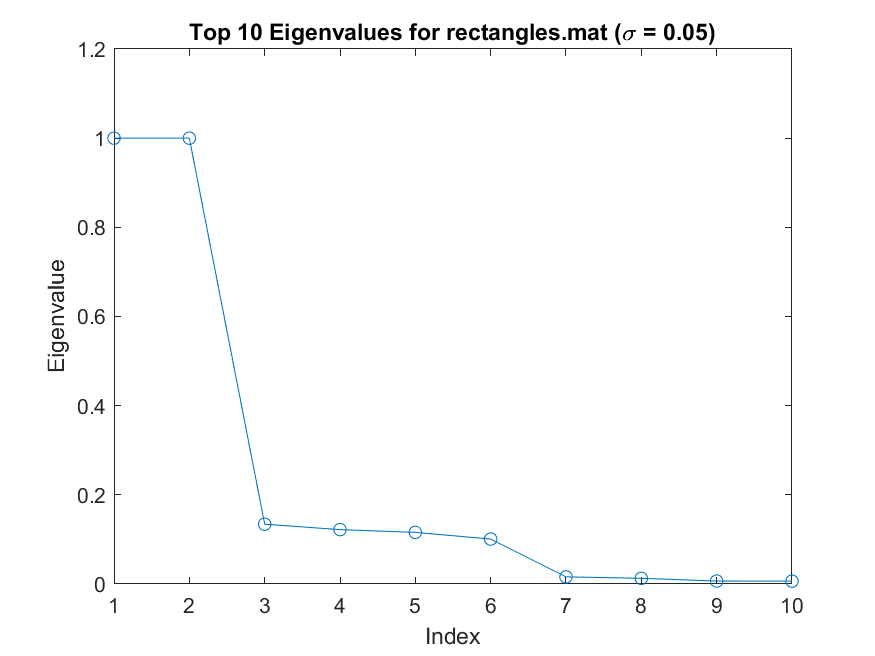
\includegraphics[width=\linewidth]{first_10_eigenvalues_rectangles.mat.png}
        \caption{\texttt{rectangles.mat}}
    \end{subfigure}
    \begin{subfigure}{0.45\textwidth}
        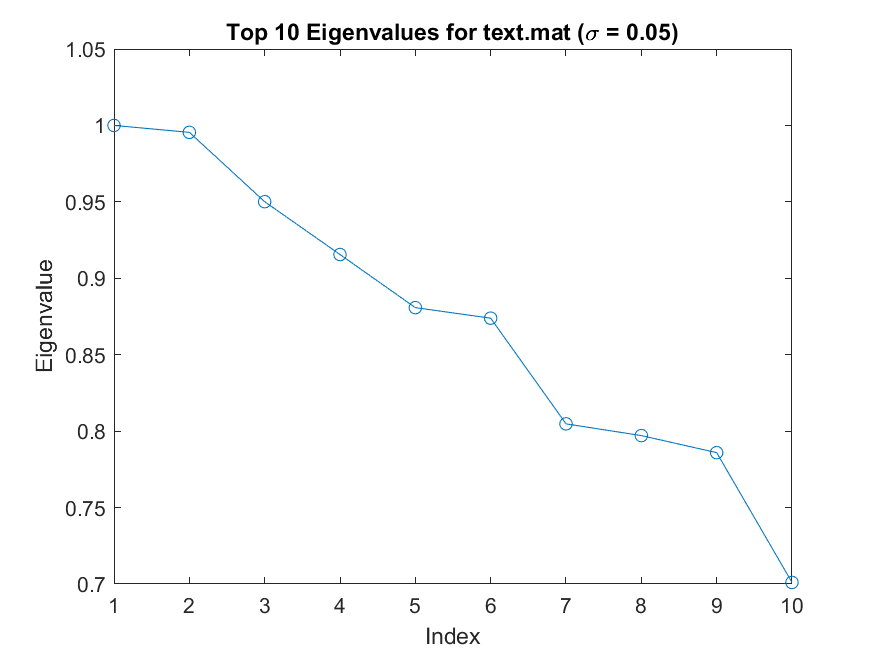
\includegraphics[width=\linewidth]{first_10_eigenvalues_text.mat.png}
        \caption{\texttt{text.mat}}
    \end{subfigure}
    \caption{First 10 eigenvalues for \texttt{rectangles.mat} and \texttt{text.mat} with \(\sigma = 0.05\).}
    \label{fig:rectangles}
\end{figure}

\textcolor{red}{P1.4, Answer:}\\

The comparison between \( k \)-means and spectral clustering contain advantages and limitations for each method based on the dataset's characteristics. 
\( k \)-means assumes that clusters are convex and roughly spherical in Euclidean space, which makes it effective for datasets like \texttt{rectangles.mat}, 
where clusters are well-separated and aligned with Euclidean distance. However, \( k \)-means struggles with datasets like \texttt{concentric.mat} and \texttt{links.mat},
where clusters are non-convex or intertwined.

Spectral clustering, on the other hand, does not rely on such assumptions and performs well with non-linear or complex cluster shapes. 
By leveraging the graph-based affinity matrix, spectral clustering captures relationships between points more effectively, making it suitable for datasets like \texttt{concentric.mat} and \texttt{links.mat}.
On the \texttt{rectangles.mat} dataset, both \( k \)-means and spectral clustering perform well because the clusters are linearly separable and geometrically simple. For \texttt{concentric.mat}, 
\( k \)-means fails because the clusters are circular and cannot be separated using straight lines, while spectral clustering identifies the circular clusters accurately. 

Similarly, on the \texttt{links.mat} dataset, \( k \)-means struggles due to the intertwined structure of the clusters, whereas spectral clustering handles the dataset effectively. On the \texttt{text.mat} dataset, 
\( k \)-means provides reasonable clustering but may struggle if clusters overlap or are not spherical. Spectral clustering, in contrast, offers better separation, especially for complex or overlapping clusters.

Regarding parameter sensitivity, \( k \)-means requires the number of clusters (\( k \)) to be specified explicitly and is sensitive to the initialization of cluster centroids, 
which can lead to different results across runs. Spectral clustering relies on the choice of the similarity function and the parameter \(\sigma\). The eigenvalue spectrum in spectral clustering provides 
insights into the optimal number of clusters, which can be an advantage in some contexts. 


\clearpage

\appendix

\section{Appendix: MATLAB Code}
\subsection{Homework 6.1}

\begin{lstlisting}[language = matlab]
    clear all
    close all
    clc

    datasets = {'text.mat', 'concentric.mat', 'links.mat', 'rectangles.mat'};
    data_vars = {'X4', 'X1', 'X3', 'X2'}; % Variable names in the .mat files

    for i = 1:length(datasets)
        load(datasets{i});
        var_name = data_vars{i};
        if exist(var_name, 'var')
            data = eval(var_name); 
        else
            error(['Variable ', var_name, ' not found in dataset ', datasets{i}]);
        end


        if strcmp(datasets{i}, 'text.mat')
            k = 6; 
        else
            k = 2; 
        end

        [idx, ~] = kmeans(data, k);

        plotClusters(data, idx);
        title(['K-means Clustering for ', datasets{i}, ', k = ', num2str(k)]);
        filename = sprintf('k_means_clustering_%s.png', datasets{i}); 
        saveas(gcf, filename);
    end
\end{lstlisting}

\subsection{Homework 6.2}

\begin{lstlisting}[language = matlab]
    clear all
    close all
    clc

    datasets = {'text.mat', 'concentric.mat', 'links.mat', 'rectangles.mat'};
    data_vars = {'X4', 'X1', 'X3', 'X2'};
    dataset_names = {'text', 'concentric', 'links', 'rectangles'}; 
    sigma_values = [0.025, 0.05, 0.2, 0.5];

    for i = 1:length(datasets)
        load(datasets{i});
        var_name = data_vars{i};
        if exist(var_name, 'var')
            data = eval(var_name); 
        else
            error(['Variable ', var_name, ' not found in dataset ', datasets{i}]);
        end

        if strcmp(datasets{i}, 'text.mat')
            k = 6; 
        else
            k = 2; 
        end

        for j = 1:length(sigma_values)
            sigma = sigma_values(j);
            idx = spectralClustering(data, k, sigma);
    
            plotClusters(data, idx);
            title(['Spectral Clustering for ', datasets{i}, ', \sigma = ', num2str(sigma)]);
            
            filename = sprintf('%s_sigma_%.3f.png', dataset_names{i}, sigma);
            saveas(gcf, filename);
        end
    end

    function [idx] = spectralClustering(data, k, sigma)
        n = size(data, 1);
        A = zeros(n, n);
        for i = 1:n
            for j = 1:n
                A(i, j) = exp(-norm(data(i, :) - data(j, :))^2 / sigma);
            end
        end

        D = diag(1 ./ sqrt(sum(A, 2)));
        N = D * A * D; 

        [V, ~] = eigs(N, k);
        Y = V ./ vecnorm(V, 2, 2);
        [idx, ~] = kmeans(Y, k);
    end

\end{lstlisting}

\subsection{Homework 6.3}
\begin{lstlisting}[language = matlab]
clear all
close all
clc

datasets = {'rectangles.mat', 'text.mat'};
data_vars = {'X2', 'X4'}; 
sigma = 0.05; 

for i = 1:length(datasets)
    load(datasets{i});
    var_name = data_vars{i};
    if exist(var_name, 'var')
        data = eval(var_name); 
    else
        error(['Variable ', var_name, ' not found in dataset ', datasets{i}]);
    end

    n = size(data, 1);
    A = zeros(n, n);
    for p = 1:n
        for q = 1:n
            A(p, q) = exp(-norm(data(p, :) - data(q, :))^2 / sigma);
        end
    end

    D = diag(1 ./ sqrt(sum(A, 2)));
    N = D * A * D;

    [V, E] = eig(N); 
    eigenvalues = diag(E); 
    eigenvalues = sort(eigenvalues, 'descend');

    figure;
    plot(1:10, eigenvalues(1:10), '-o');
    title(['Top 10 Eigenvalues for ', datasets{i}, ' (\sigma = 0.05)']);
    xlabel('Index');
    ylabel('Eigenvalue');
    filename = sprintf('first_10_eigenvalues_%s.png', datasets{i}); 
    saveas(gcf, filename);
end

\end{lstlisting}

\end{document}
